\documentclass[
  paper=a4,
  % version=3.25,
  pagesize=pdftex,
  twoside=false,
  toc=listof,
  BCOR=0pt,
  DIV=15,
  indent,
]{scrartcl}
\usepackage{pdfpages}
\usepackage[margin=5mm]{geometry}
\usepackage{ctex}
\usepackage{tcolorbox}
\usepackage{pdfpages}
\usepackage{tikz-network}
\usepackage{tikz-documentation}
\usepackage{xcolor}
\pagecolor{lightgray!15}

\renewcommand{\lstlistlistingname}{Codeverzeichnis}
\renewcommand{\lstlistingname}{Quellcode}
% \lstset{caption=\lstname}

% Globale Einstellungen
\lstdefinestyle{latex}{
language=[AlLaTeX]TeX,
extendedchars=true,
frame=single,
keepspaces=true,
backgroundcolor=\color{pink!8!white},
rulecolor=\color{red},
breaklines=true,
% xleftmargin=\parindent,
basicstyle=\footnotesize\ttfamily,
keywordstyle=\bfseries\color{blue},
commentstyle=\itshape\color{gray},
identifierstyle=\bfseries\color{magenta},
stringstyle=\color{orange},
}
%=================================
% Globale Einstellungen
\usepackage{accsupp}
%% Nummern nicht auswählbar machen
\newcommand{\noncopynumber}[1]{ \BeginAccSupp{method=escape,ActualText={}}
#1
\EndAccSupp{}}%
%%

\lstset {numberstyle=\tiny\color{gray!90!black}\noncopynumber,
numbers=left,
numbersep=2pt,
columns=flexible,
title=\bfseries
}


\newcommand{\MS}{Martin Scheidt}

\hypersetup{
  pdftitle={tikz/networkmanual},
  pdfsubject={A tikz toolbox for track schematics},
  pdfauthor={Latex Studio},
  pdfkeywords={latex, tikz, library, railway, track, layout}
}

%% 2.1

\def\firstcircle{ (0.0, 0.0) circle (1.5)}
\def\secondcircle{(2.0, 0.0) circle (1.5)}
\def\thirdcircle{ (1.0,-1.5) circle (1.5)}
\def\rectangle{ (-1.5,-3.0) rectangle (3.5,1.0) }
\colorlet{circle edge}{black}
\colorlet{circle area}{blue!20}
\tikzset{filled/.style={fill=circle area, draw=circle edge, thick},
    outline/.style={draw=circle edge, thick}}
\setlength{\parskip}{5mm}
%% 2.2

\usetikzlibrary{patterns}

\def\radius{1cm}
\def\ratio{0.8}

\def\circleA{(90:\ratio*\radius) circle [radius=\radius]}
\def\circleB{(-150:\ratio*\radius) circle [radius=\radius]}
\def\circleC{(-30:\ratio*\radius) circle [radius=\radius]}

\tikzset{set label/.style={fill=white,circle,inner sep=.5mm}}

\def\drawLabels{%
  \node[set label] at (90:\radius+\ratio*\radius) {A};
  \node[set label] at (-150:\radius+\ratio*\radius) {B};
  \node[set label] at (-30:\radius+\ratio*\radius) {C};
}
\def\drawCaption#1{\node at (-90:2*\radius) {$#1$};}

\def\drawVenn#1#2{
  \begin{tikzpicture}[baseline=0pt]
    \path[use as bounding box] (0,0) circle [radius=2.5*\radius];
    \draw \circleA \circleB \circleC;
    \begin{scope}[pattern=north west lines,pattern color=blue]
      #2
    \end{scope}
    \drawLabels
    \drawCaption{#1}
  \end{tikzpicture}%
}

\graphicspath{{figures/}}
\allowdisplaybreaks

\begin{document}


\title{\tikz\node[scale=1.2]{\color{gray}\Huge\sffamily \{\textcolor{black}{Ti\textcolor{red}{\emph{k}}Z}/\textcolor{blue}{PGF}\textcolor{green!40!black}{plots}~常用图形绘制合集\}};}
\subtitle{Ti\emph{k}Z \textcolor{orange}{\&} PGF \textcolor{blue}{那些年,我们一直没画好的图像}}
\author{\vhListAllAuthorsLong}
\date{Version \vhCurrentVersion~ from \vhCurrentDate}
\thispagestyle{empty}
\maketitle

\cleardoublepage

\thispagestyle{empty}
\begin{multicols}{2}
  \tableofcontents
\end{multicols}

\cleardoublepage

\section{内容说明}
\label{sec:intro}

这部分内容是我收集的在中学学习阶段教师用到的常见的作图。资源来源于诸多作者如\href{https://yuxtech.github.io/2020/04/05/tikz/}{向禹老师}、\href{https://www.latexstudio.net/index/details/index/mid/1047.html}{Banach Spaces}、\href{http://latexstudio.net}{latexstudio}等。

\newpage

\section{集合部分的常用图形(Venn 图)的~TikZ 实现}

\subsection{集合关系的~Venn 图}
\begin{enumerate}
  \item 两个集合的交集

  \begin{minipage}[c]{0.51\textwidth}
  \centering
  \begin{lstlisting}[gobble=0]
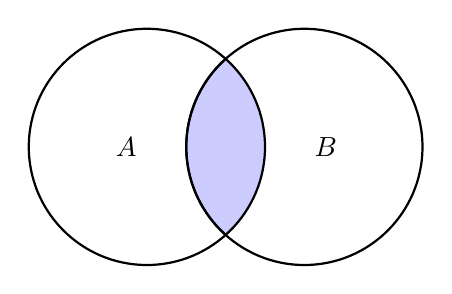
\begin{tikzpicture}
    \begin{scope}
        \clip \firstcircle;
        \fill[filled] \secondcircle;
    \end{scope}
    \draw[outline] \firstcircle  node[left]  {$A$};
    \draw[outline] \secondcircle node[right] {$B$};
\end{tikzpicture}
  \end{lstlisting}
\end{minipage}
\hfil
\begin{minipage}[c]{0.45\textwidth}
  \centering
  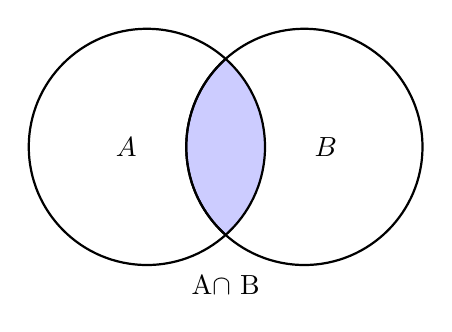
\begin{tikzpicture}
    \begin{scope}
        \clip \firstcircle;
        \fill[filled] \secondcircle;
    \end{scope}
    \draw[outline] \firstcircle  node[left]  {$A$};
    \draw[outline] \secondcircle node[right] {$B$};
     \node[anchor=north,align=center] at (current bounding box.south)
      {A$\cap$ B};
\end{tikzpicture}
\end{minipage}

 \begin{minipage}[c]{0.6\textwidth}
   \lstinputlisting[style=latex, firstline=17,lastline=26]{figures/AcapB.tex}
\end{minipage}
\hfil
\begin{minipage}[c]{0.35\textwidth}
  \centering
 \includegraphics[width=\linewidth]{AcapB}
\end{minipage}


 \item 三个集合的交集

  \begin{minipage}[c]{0.51\textwidth}
  \centering
  \begin{lstlisting}[gobble=0]
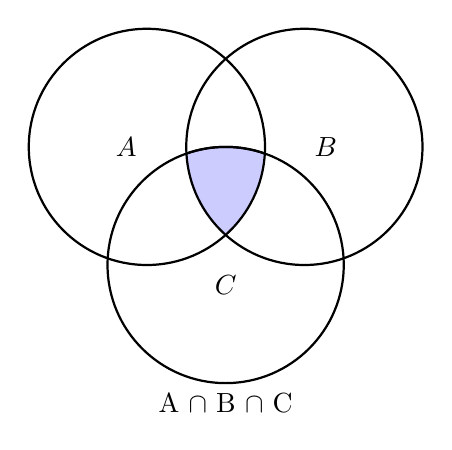
\begin{tikzpicture}
    \begin{scope}
        \clip  \firstcircle;
        \clip  \secondcircle;
        \fill[filled]   \thirdcircle ;
    \end{scope}
    \draw[outline] \firstcircle  node[left]  {$A$};
    \draw[outline] \secondcircle node[right] {$B$};
    \draw[outline] \thirdcircle  node[below] {$C$};
    \node[anchor=north] at (current bounding box.south) {A $\cap$ B $\cap$ C};
\end{tikzpicture}
  \end{lstlisting}
\end{minipage}
\hfil
\begin{minipage}[c]{0.45\textwidth}
  \centering
  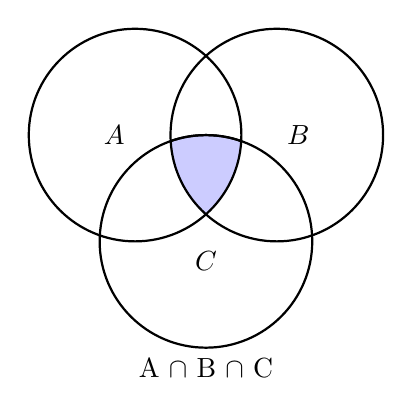
\begin{tikzpicture}[scale=0.9]
    \begin{scope}
        \clip  \firstcircle;
        \clip  \secondcircle;
        \fill[filled]   \thirdcircle ;
    \end{scope}
    \draw[outline] \firstcircle  node[left]  {$A$};
    \draw[outline] \secondcircle node[right] {$B$};
    \draw[outline] \thirdcircle  node[below] {$C$};
    \node[anchor=north] at (current bounding box.south) {A $\cap$ B $\cap$ C};
\end{tikzpicture}
\end{minipage}

\item 两个集合的并集

  \begin{minipage}[c]{0.51\textwidth}
  \centering
  \begin{lstlisting}[gobble=0]
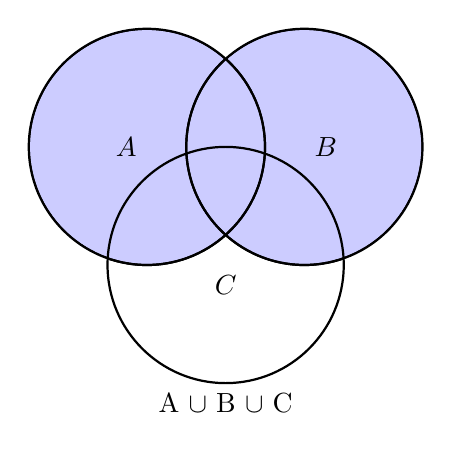
\begin{tikzpicture}
    \begin{scope}
        \clip \firstcircle \secondcircle \thirdcircle;
        \fill[filled]  \firstcircle \secondcircle;
    \end{scope}
    \draw[outline] \firstcircle  node[left]  {$A$};
    \draw[outline] \secondcircle node[right] {$B$};
    \draw[outline] \thirdcircle  node[below] {$C$};
    \node[anchor=north] at (current bounding box.south) {A $\cup$ B $\cup$ C};
\end{tikzpicture}
  \end{lstlisting}
\end{minipage}
\hfil
\begin{minipage}[c]{0.45\textwidth}
  \centering
  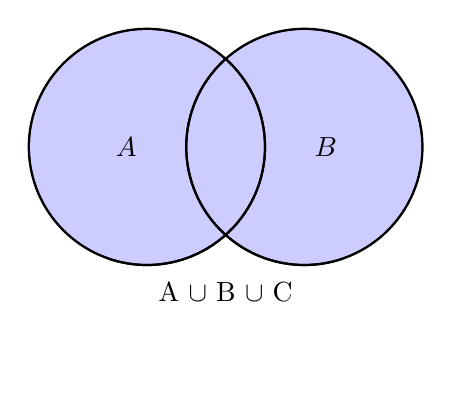
\begin{tikzpicture}
    \begin{scope}
        \clip \firstcircle \secondcircle \thirdcircle;
        \fill[filled]  \firstcircle \secondcircle;
    \end{scope}
    \draw[outline] \firstcircle  node[left]  {$A$};
    \draw[outline] \secondcircle node[right] {$B$};
    \node[anchor=north] at ($(current bounding box.south)+(0pt,40pt)$) {A $\cup$ B $\cup$ C};
\end{tikzpicture}
\end{minipage}

\item 三个集合的并集

  \begin{minipage}[c]{0.51\textwidth}
  \centering
  \begin{lstlisting}[gobble=0]
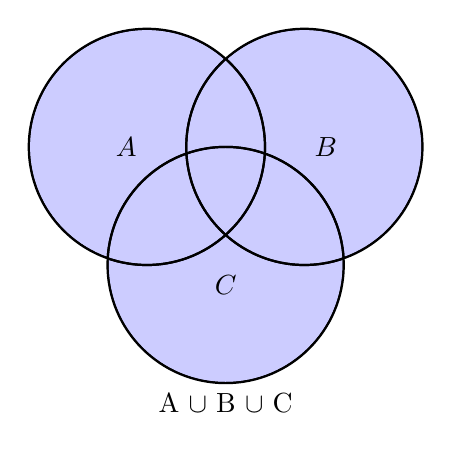
\begin{tikzpicture}
    \begin{scope}
        \clip \firstcircle \secondcircle \thirdcircle;
        \fill[filled]  \firstcircle \secondcircle \thirdcircle;
    \end{scope}
    \draw[outline] \firstcircle  node[left]  {$A$};
    \draw[outline] \secondcircle node[right] {$B$};
    \draw[outline] \thirdcircle  node[below] {$C$};
    \node[anchor=north] at (current bounding box.south) {A $\cup$ B $\cup$ C};
\end{tikzpicture}
  \end{lstlisting}
\end{minipage}
\hfil
\begin{minipage}[c]{0.45\textwidth}
  \centering
  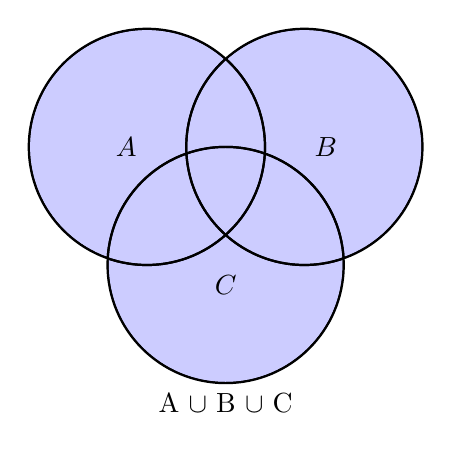
\begin{tikzpicture}
    \begin{scope}
        \clip \firstcircle \secondcircle \thirdcircle;
        \fill[filled]  \firstcircle \secondcircle \thirdcircle;
    \end{scope}
    \draw[outline] \firstcircle  node[left]  {$A$};
    \draw[outline] \secondcircle node[right] {$B$};
    \draw[outline] \thirdcircle  node[below] {$C$};
    \node[anchor=north] at (current bounding box.south) {A $\cup$ B $\cup$ C};
\end{tikzpicture}
\end{minipage}

\begin{minipage}[c]{0.6\textwidth}
   \lstinputlisting[style=latex, firstline=30,lastline=39]{figures/ABC.tex}
\end{minipage}
\hfil
\begin{minipage}[c]{0.35\textwidth}
  \centering
 \includegraphics[width=\linewidth]{ABC}
\end{minipage}


\item 两个集合的并集与第三个集合的交集

  \begin{minipage}[c]{0.51\textwidth}
  \centering
  \begin{lstlisting}[gobble=0]
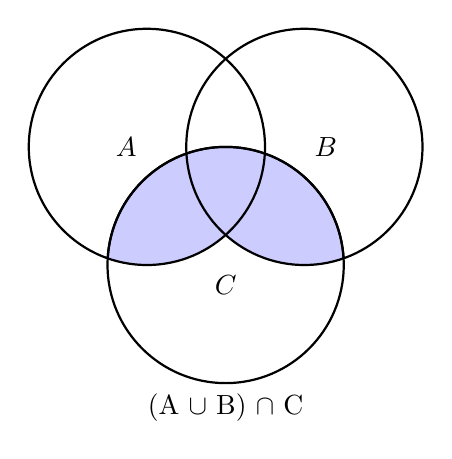
\begin{tikzpicture}
     \begin{scope}
        \clip \firstcircle \secondcircle;
        \fill[filled] \thirdcircle;
    \end{scope}
    \draw[outline] \firstcircle  node[left]  {$A$};
    \draw[outline] \secondcircle node[right] {$B$};
    \draw[outline] \thirdcircle  node[below] {$C$};
    \node[anchor=north] at (current bounding box.south)
      {(A $\cup$ B) $\cap$ C};
\end{tikzpicture}
  \end{lstlisting}
\end{minipage}
\hfil
\begin{minipage}[c]{0.45\textwidth}
  \centering
  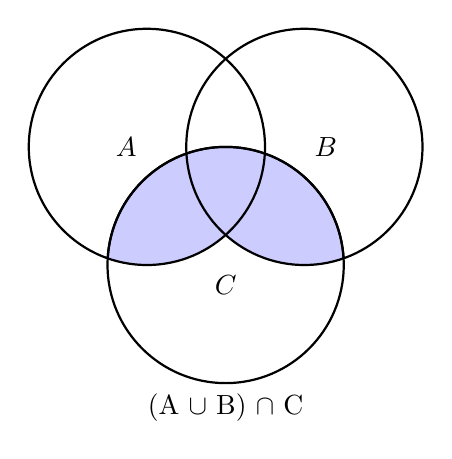
\begin{tikzpicture}
     \begin{scope}
        \clip \firstcircle \secondcircle;
        \fill[filled] \thirdcircle;
    \end{scope}
    \draw[outline] \firstcircle  node[left]  {$A$};
    \draw[outline] \secondcircle node[right] {$B$};
    \draw[outline] \thirdcircle  node[below] {$C$};
    \node[anchor=north] at (current bounding box.south)
      {(A $\cup$ B) $\cap$ C};
\end{tikzpicture}
\end{minipage}


\item 两个集合的交集并上第三个集合

  \begin{minipage}[c]{0.51\textwidth}
  \centering
  \begin{lstlisting}[gobble=0]
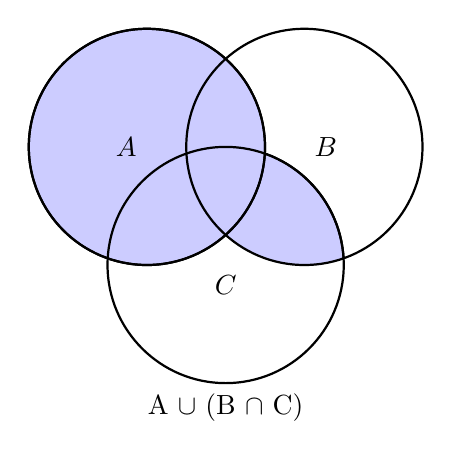
\begin{tikzpicture}
     \begin{scope}
        \clip \secondcircle;
        \fill[filled] \thirdcircle;
    \end{scope}
    \fill[filled]  \firstcircle;
    \draw[outline] \firstcircle  node[left]  {$A$};
    \draw[outline] \secondcircle node[right] {$B$};
    \draw[outline] \thirdcircle  node[below] {$C$};
    \node[anchor=north] at (current bounding box.south)
      {A $\cup$ (B $\cap$ C)};
\end{tikzpicture}
  \end{lstlisting}
\end{minipage}
\hfil
\begin{minipage}[c]{0.45\textwidth}
  \centering
  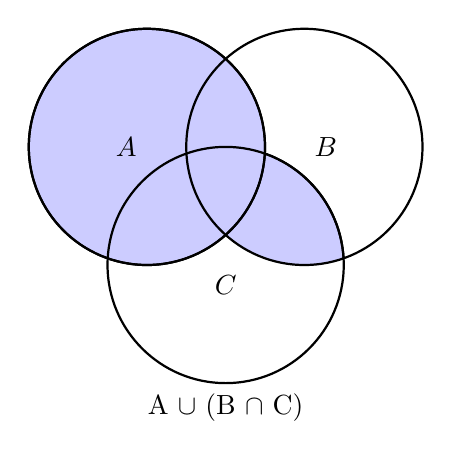
\begin{tikzpicture}
     \begin{scope}
        \clip \secondcircle;
        \fill[filled] \thirdcircle;
    \end{scope}
    \fill[filled]  \firstcircle;
    \draw[outline] \firstcircle  node[left]  {$A$};
    \draw[outline] \secondcircle node[right] {$B$};
    \draw[outline] \thirdcircle  node[below] {$C$};
    \node[anchor=north] at (current bounding box.south)
      {A $\cup$ (B $\cap$ C)};
\end{tikzpicture}
\end{minipage}

\item 两个集合的补集的交交上第三个集合

  \begin{minipage}[c]{0.51\textwidth}
  \centering
  \begin{lstlisting}[gobble=0]
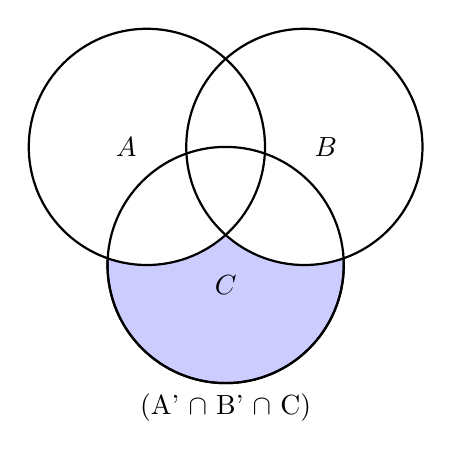
\begin{tikzpicture}
    \begin{scope}
        \fill[filled] \thirdcircle;
        \fill[white]  \firstcircle;
        \fill[white]  \secondcircle;
    \end{scope}
    \draw[outline] \firstcircle  node[left]  {$A$};
    \draw[outline] \secondcircle node[right] {$B$};
    \draw[outline] \thirdcircle  node[below] {$C$};
    \node[anchor=north] at (current bounding box.south)
      {(A' $\cap$ B' $\cap$ C)};
      \end{tikzpicture}
  \end{lstlisting}
\end{minipage}
\hfil
\begin{minipage}[c]{0.45\textwidth}
  \centering
  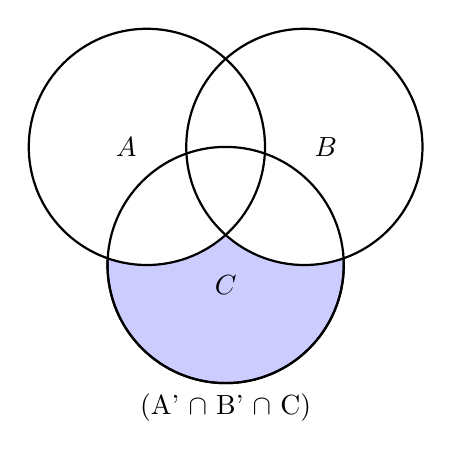
\begin{tikzpicture}
    \begin{scope}
        \fill[filled] \thirdcircle;
        \fill[white]  \firstcircle;
        \fill[white]  \secondcircle;
    \end{scope}
    \draw[outline] \firstcircle  node[left]  {$A$};
    \draw[outline] \secondcircle node[right] {$B$};
    \draw[outline] \thirdcircle  node[below] {$C$};
    \node[anchor=north] at (current bounding box.south)
      {(A' $\cap$ B' $\cap$ C)};
      \end{tikzpicture}
\end{minipage}

\end{enumerate}

\subsection{集合运算的~Venn 图表示}

\begin{minipage}[c]{0.51\textwidth}
  \centering
  \begin{lstlisting}[gobble=0]
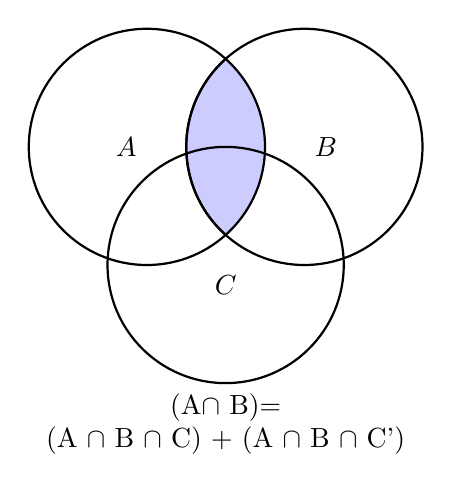
\begin{tikzpicture}
    \begin{scope}
        \clip \firstcircle;
        \fill[filled] \secondcircle;
    \end{scope}
    \draw[outline] \firstcircle  node[left]  {$A$};
    \draw[outline] \secondcircle node[right] {$B$};
    \draw[outline] \thirdcircle  node[below] {$C$};
    \node[anchor=north,align=center] at (current bounding box.south)
      {(A$\cap$ B)=\\(A $\cap$ B $\cap$ C) + (A $\cap$ B $\cap$ C')};
\end{tikzpicture}
  \end{lstlisting}
\end{minipage}
\hfil
\begin{minipage}[c]{0.45\textwidth}
  \centering
  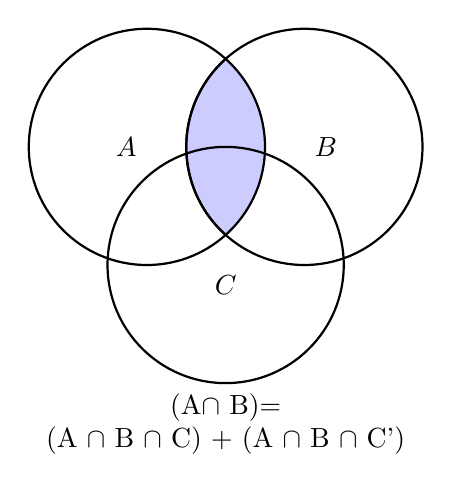
\begin{tikzpicture}
    \begin{scope}
        \clip \firstcircle;
        \fill[filled] \secondcircle;
    \end{scope}
    \draw[outline] \firstcircle  node[left]  {$A$};
    \draw[outline] \secondcircle node[right] {$B$};
    \draw[outline] \thirdcircle  node[below] {$C$};
    \node[anchor=north,align=center] at (current bounding box.south)
      {(A$\cap$ B)=\\(A $\cap$ B $\cap$ C) + (A $\cap$ B $\cap$ C')};
\end{tikzpicture}
\end{minipage}

\begin{align*}
&
\drawVenn{(A\cup B)\cap C}{\clip \circleC; \fill \circleA; \fill \circleB;}
\mathrel{\scalebox{2}{$=$}}
\drawVenn{A\cap C}{\clip \circleC; \fill \circleA;}
\mathbin{\scalebox{2}{$\cup$}}
\drawVenn{B\cap C}{\clip \circleB; \fill \circleC;}\\
&
\drawVenn{(A\cap B)\cup C}{\clip \circleC \circleA; \fill \circleB; \fill \circleC;}
\mathrel{\scalebox{2}{$=$}}
\drawVenn{A\cup C}{\fill \circleC; \fill \circleA;}
\mathbin{\scalebox{2}{$\cap$}}
\drawVenn{B\cup C}{\fill \circleB; \fill \circleC;}
\end{align*}

 \lstinputlisting[style=latex, firstline=1]{figures/Sets1.tex}
 
\begin{minipage}[c]{0.485\linewidth}
\includegraphics[width=\linewidth]{Sets1}
\end{minipage}
\hfill
\begin{minipage}[c]{0.4\linewidth}
   \centering
 \includegraphics[width=\linewidth]{Sets2}
\end{minipage}

   \lstinputlisting[style=latex, firstline=1,lastline=63]{figures/Sets2.tex}

   \lstinputlisting[style=latex, firstline=1]{figures/Sets.tex}


\begin{minipage}[c]{0.485\linewidth}
  \centering
 \includegraphics[width=\linewidth]{Setsa}
\end{minipage}\hfill
\begin{minipage}[c]{0.485\linewidth}
  \centering
 \includegraphics[width=\linewidth]{Sets}
\end{minipage}

\section{常见函数图像的~TikZ 实现}

\subsection{常用函数的~TikZ 绘制}

\begin{enumerate}
  \item 一次函数

  \begin{minipage}[c]{0.51\textwidth}
  \centering
  \begin{lstlisting}[gobble=0]
  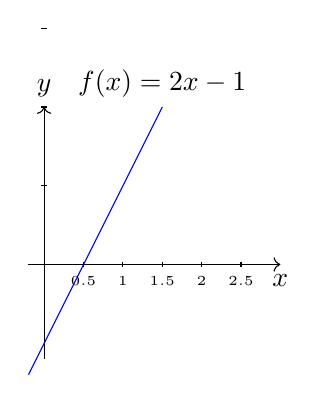
\begin{tikzpicture}
    \draw[->](-0.2,0)--(3,0) node[below] {$x$};
    \draw[->](0,-1.2)--(0,2) node[above] {$y$};
    \draw[domain=-0.2:1.5,draw=blue] plot (\x,{2*\x-1}) node[above] {$f(x)=2x-1$};
    \foreach \x in {0.5,1,...,2.5}
   \draw (\x cm,1pt) -- (\x cm,-1pt) node[anchor=north] {\tiny $\x $};
\foreach \y in {1,2,3}
\draw (1pt,\y cm) -- (-1pt,\y cm);
\end{tikzpicture}
  \end{lstlisting}
\end{minipage}
\hfil
\begin{minipage}[c]{0.45\textwidth}
  \centering
  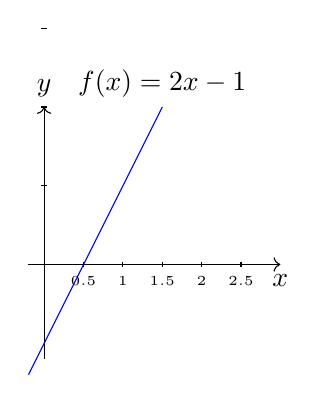
\begin{tikzpicture}
    \draw[->](-0.2,0)--(3,0) node[below] {$x$};
    \draw[->](0,-1.2)--(0,2) node[above] {$y$};
    \draw[domain=-0.2:1.5,draw=blue] plot (\x,{2*\x-1}) node[above] {$f(x)=2x-1$};
    \foreach \x in {0.5,1,...,2.5}
   \draw (\x cm,1pt) -- (\x cm,-1pt) node[anchor=north] {\tiny $\x $};
\foreach \y in {1,2,3}
\draw (1pt,\y cm) -- (-1pt,\y cm);
\end{tikzpicture}
\end{minipage}

\item 二次函数

\begin{minipage}[c]{0.51\textwidth}
  \centering
  \begin{lstlisting}[gobble=0]
  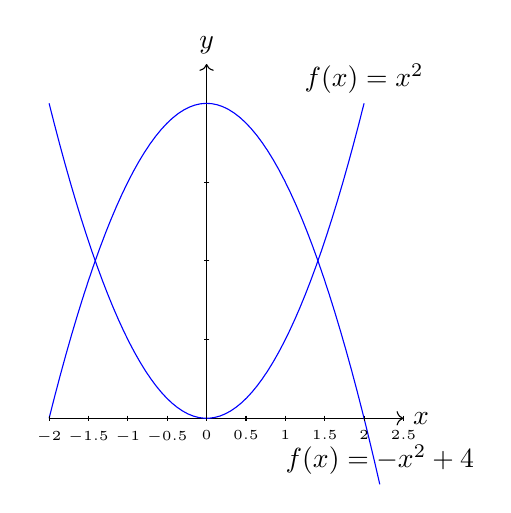
\begin{tikzpicture}
    \draw[->](-2,0)--(2.5,0) node[right] {$x$};
    \draw[->](0,0)--(0,4.5) node[above] {$y$};
    \draw[domain=-2:2,draw=blue,samples=60] plot (\x,{(\x)^2}) node[above] {$f(x)=x^2$};
    \draw[domain=-2:2.2,draw=blue,samples=60] plot (\x,{-(\x)^2+4}) node[above] {$f(x)=-x^2+4$};
    \foreach \x in {-2,-1.5,...,2.5}
   \draw (\x cm,1pt) -- (\x cm,-1pt) node[anchor=north] {\tiny $\x $};
\foreach \y in {1,2,3}
\draw (1pt,\y cm) -- (-1pt,\y cm);
\end{tikzpicture}
  \end{lstlisting}
\end{minipage}
\hfil
\begin{minipage}[c]{0.45\textwidth}
  \centering
  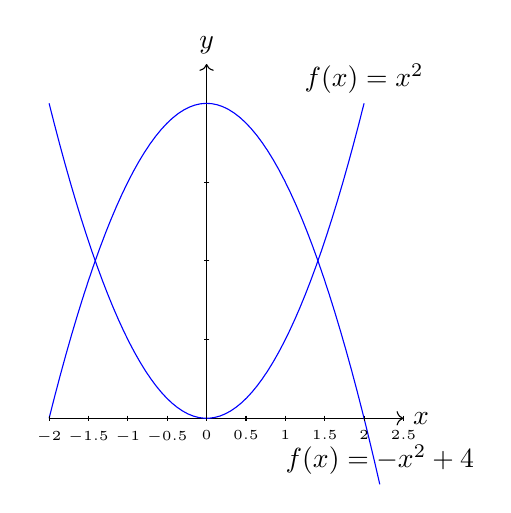
\begin{tikzpicture}
    \draw[->](-2,0)--(2.5,0) node[right] {$x$};
    \draw[->](0,0)--(0,4.5) node[above] {$y$};
    \draw[domain=-2:2,draw=blue,samples=60] plot (\x,{(\x)^2}) node[above] {$f(x)=x^2$};
    \draw[domain=-2:2.2,draw=blue,samples=60] plot (\x,{-(\x)^2+4}) node[above] {$f(x)=-x^2+4$};
    \foreach \x in {-2,-1.5,...,2.5}
   \draw (\x cm,1pt) -- (\x cm,-1pt) node[anchor=north] {\tiny $\x $};
\foreach \y in {1,2,3}
\draw (1pt,\y cm) -- (-1pt,\y cm);
\end{tikzpicture}
\end{minipage}

\item 多次函数

\begin{minipage}[c]{0.51\textwidth}
  \centering
  \begin{lstlisting}[gobble=0]
  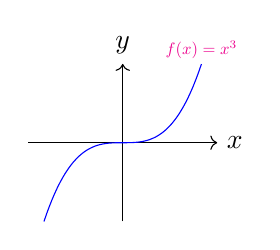
\begin{tikzpicture}
    \draw[->](-1.2,0)--(1.2,0) node[right] {$x$};
    \draw[->](0,-1)--(0,1) node[above] {$y$};
    \draw[domain=-1:1,draw=blue,samples=60] plot (\x,{(\x)^3}) node[above,scale=0.6,color=magenta] {$f(x)=x^3$};
\end{tikzpicture}
  \end{lstlisting}
\end{minipage}
\hfil
\begin{minipage}[c]{0.45\textwidth}
  \centering
\begin{tikzpicture}[scale=2]
    \draw[->](-1,0)--(2,0) node[right] {$x$};
    \draw[->](0,-1)--(0,1) node[above] {$y$};
    \draw[domain=-0.5:1.5,draw=blue,samples=60] plot (\x,{(\x-0.5)^3}) node[above,scale=0.6,color=magenta] {$f(x)=(x-0.5)^3$};
    \draw[domain=-1:1,draw=yellow,samples=60] plot (\x,{(\x)^4-0.5})
    node[above,scale=0.6,color=yellow] {$f(x)=x^4-0.5$};
\end{tikzpicture}
\end{minipage}

\lstinputlisting[style=latex, firstline=6,lastline=23]{figures/Foncations.tex}
\begin{minipage}[c]{0.4\linewidth}
  \centering
 \includegraphics[width=\linewidth]{Foncations}
\end{minipage}


\end{enumerate}

\subsection{指数函数图像的~TikZ 绘制}

\begin{minipage}[c]{0.485\textwidth}
  \centering
  \begin{lstlisting}[gobble=0]
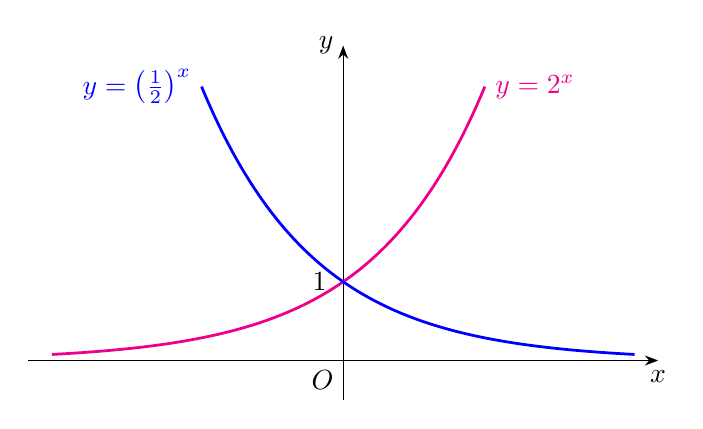
\begin{tikzpicture}[samples=100]
\draw[-Stealth](-4,0)--(0,0)node[below left]{$O$}--(4,0)node[below]{$x$};
\draw[-Stealth](0,-0.5)--(0,4)node[left]{$y$};
\draw[domain=-3.7:1.8,line width=1pt,draw=magenta]plot(\x,{2^(\x)})node[right,color=magenta]{$y=2^x$};
\draw[domain=3.7:-1.8,line width=1pt,draw=blue]plot(\x,{2^(-\x)})node[left,color=blue]{$y=\left(\frac12\right)^x$};
\node at(-0.3,1){$1$};
\end{tikzpicture}
  \end{lstlisting}
\end{minipage}
\hfil
\begin{minipage}[c]{0.45\textwidth}
  \centering
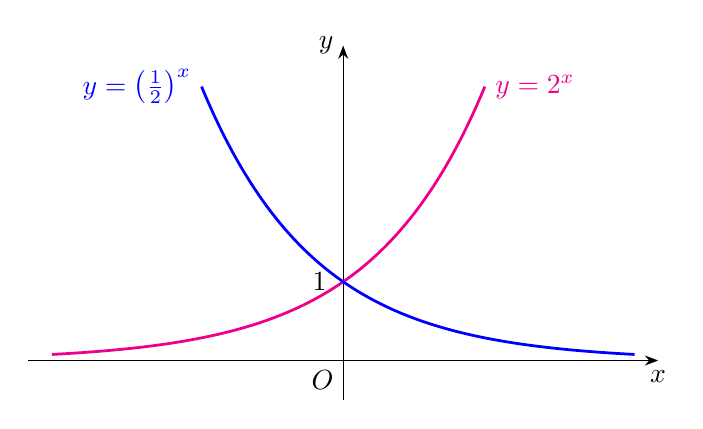
\begin{tikzpicture}[samples=100]
\draw[-Stealth](-4,0)--(0,0)node[below left]{$O$}--(4,0)node[below]{$x$};
\draw[-Stealth](0,-0.5)--(0,4)node[left]{$y$};
\draw[domain=-3.7:1.8,line width=1pt,draw=magenta]plot(\x,{2^(\x)})node[right,color=magenta]{$y=2^x$};
\draw[domain=3.7:-1.8,line width=1pt,draw=blue]plot(\x,{2^(-\x)})node[left,color=blue]{$y=\left(\frac12\right)^x$};
\node at(-0.3,1){$1$};
\end{tikzpicture}
\end{minipage}

\subsection{对数函数的~TikZ 图像绘制}

\begin{minipage}[c]{0.485\textwidth}
  \centering
  \begin{lstlisting}[gobble=0]
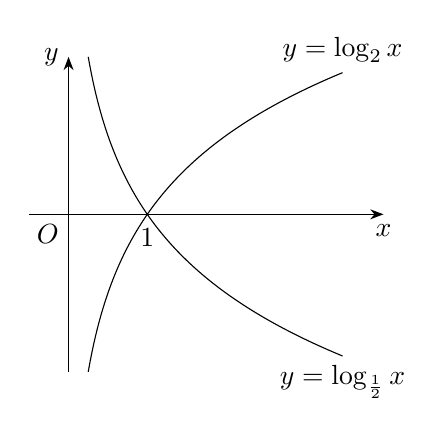
\begin{tikzpicture}[samples=100]
\draw[-Stealth](-0.5,0)--(0,0)node[below left]{$O$}
--(4,0)node[below]{$x$};
\draw[-Stealth](0,-2)
--(0,2)node[left]{$y$};
\node at(1,-0.3){$1$};
\draw[domain=-2:1.8]plot({2^(\x)},\x)
node[above]{$y=\log_2x$};
\draw[domain=2:-1.8]plot({2^(-\x)},\x)
node[below]{$y=\log_{\frac12}x$};
\end{tikzpicture}
  \end{lstlisting}
\end{minipage}
\hfil
\begin{minipage}[c]{0.45\textwidth}
  \centering
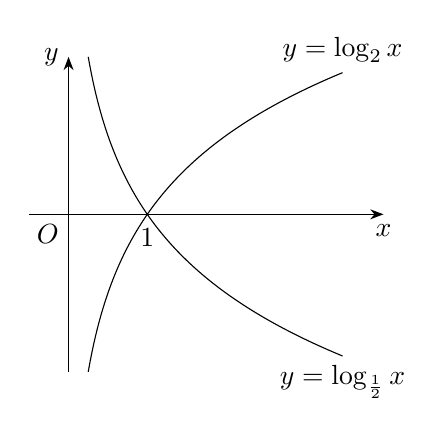
\begin{tikzpicture}[samples=100]
\draw[-Stealth](-0.5,0)--(0,0)node[below left]{$O$}--(4,0)node[below]{$x$};
\draw[-Stealth](0,-2)--(0,2)node[left]{$y$};
\node at(1,-0.3){$1$};
\draw[domain=-2:1.8]plot({2^(\x)},\x)node[above]{$y=\log_2x$};
\draw[domain=2:-1.8]plot({2^(-\x)},\x)node[below]{$y=\log_{\frac12}x$};
\end{tikzpicture}
\end{minipage}


\subsection{幂函数图像的~TikZ 绘制}
\begin{minipage}[c]{0.485\textwidth}
  \centering
  \begin{lstlisting}[gobble=0]
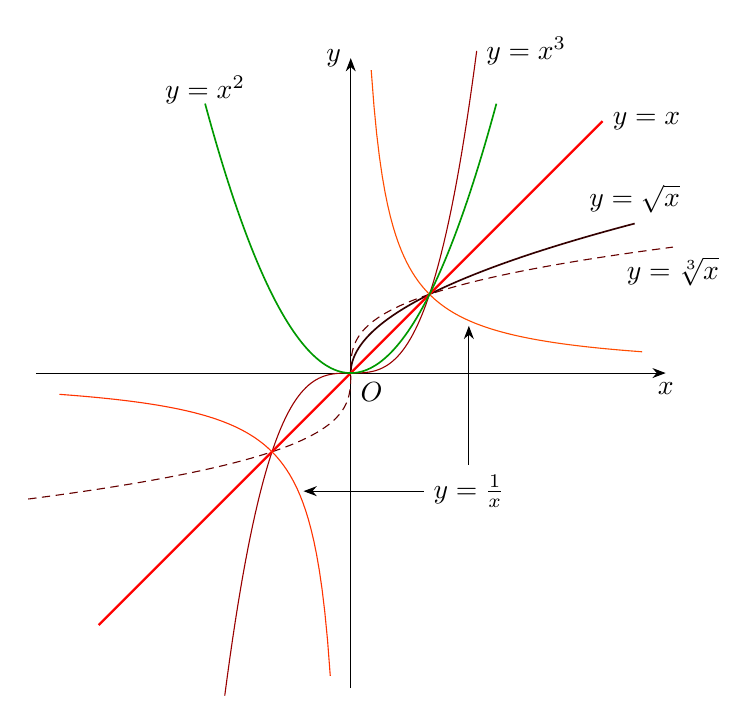
\begin{tikzpicture}[samples=100]
\draw[-Stealth](-4,0)--(0,0)node[below right]{$O$}--(4,0)node[below]{$x$};
\draw[-Stealth](0,-4)--(0,4)node[left]{$y$};
\draw[domain=-1.6:1.6,draw=red!60!black]plot(\x,{(\x)^3})node[right]{$y=x^3$};
\draw[densely dashed,domain=-1.6:1.6,draw=red!40!black]plot({(\x)^3},\x)node[below]{$y=\sqrt[3]x$};
\draw[semithick,domain=0:1.9,draw=red!20!black]plot({(\x)^2},\x)node[above]{$y=\sqrt x$};
\draw[thick,domain=-3.2:3.2,draw=red]plot(\x,\x)node[right]{$y=x$};
\draw[domain=0.26:3.7,draw=orange!60!red]plot(\x,{1/(\x)});
\draw[domain=-0.26:-3.7,draw=orange!40!red]plot(\x,{1/(\x)});
\node(a)at(1.5,-1.5){$y=\frac1x$};
\draw[-Stealth](a.west)--(-0.6,-1.5);
\draw[-Stealth](a.north)--(1.5,0.6);
\draw[semithick,domain=-1.85:1.85,draw=green!60!black]plot(\x,{(\x)^2});
\node at(-1.85,3.6){$y=x^2$};
\end{tikzpicture}
  \end{lstlisting}
\end{minipage}
\hfil
\begin{minipage}[c]{0.45\textwidth}
  \centering
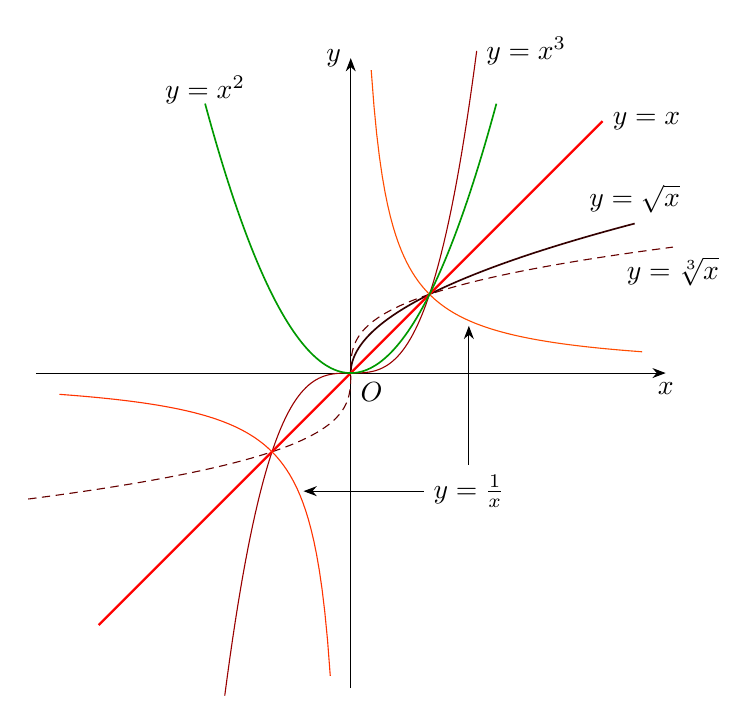
\begin{tikzpicture}[samples=100]
\draw[-Stealth](-4,0)--(0,0)node[below right]{$O$}--(4,0)node[below]{$x$};
\draw[-Stealth](0,-4)--(0,4)node[left]{$y$};
\draw[domain=-1.6:1.6,draw=red!60!black]plot(\x,{(\x)^3})node[right]{$y=x^3$};
\draw[densely dashed,domain=-1.6:1.6,draw=red!40!black]plot({(\x)^3},\x)node[below]{$y=\sqrt[3]x$};
\draw[semithick,domain=0:1.9,draw=red!20!black]plot({(\x)^2},\x)node[above]{$y=\sqrt x$};
\draw[thick,domain=-3.2:3.2,draw=red]plot(\x,\x)node[right]{$y=x$};
\draw[domain=0.26:3.7,draw=orange!60!red]plot(\x,{1/(\x)});
\draw[domain=-0.26:-3.7,draw=orange!40!red]plot(\x,{1/(\x)});
\node(a)at(1.5,-1.5){$y=\frac1x$};
\draw[-Stealth](a.west)--(-0.6,-1.5);
\draw[-Stealth](a.north)--(1.5,0.6);
\draw[semithick,domain=-1.85:1.85,draw=green!60!black]plot(\x,{(\x)^2});
\node at(-1.85,3.6){$y=x^2$};
\end{tikzpicture}
\end{minipage}


\subsection{周期函数的~TikZ 绘制}

%\includepdf[pages={1,2}]{figures/SCTfonction2.pdf} 

\subsection{其他函数图像的~TikZ 绘制}

\subsection{三角函数的~TikZ 绘制}

\subsubsection{正、余弦和正切函数}

\begin{enumerate}

  \item 正弦函数

平移

 \lstinputlisting[style=latex, firstline=12,lastline=67]{figures/Sfonction1.tex}

 \includegraphics[width=\linewidth,angle=0]{Sfonction1}

 \lstinputlisting[style=latex, firstline=12,lastline=67]{figures/Sfonction2.tex}

 \includegraphics[width=\linewidth,angle=0]{Sfonction2}

 \lstinputlisting[style=latex, firstline=12,lastline=67]{figures/Sfonction3.tex}

 \includegraphics[width=\linewidth,angle=0]{Sfonction3}

 \lstinputlisting[style=latex, firstline=38,lastline=74]{figures/Sfonction4.tex}

 \includegraphics[width=\linewidth,angle=0]{Sfonction4-1}

\lstinputlisting[style=latex, firstline=78,lastline=113]{figures/Sfonction4.tex}

 \includegraphics[width=\linewidth,angle=0]{Sfonction4-2}
 
 \lstinputlisting[style=latex, firstline=117,lastline=143]{figures/Sfonction4.tex}

 \includegraphics[width=\linewidth,angle=0]{Sfonction4-3}


 \lstinputlisting[style=latex, firstline=12,lastline=67]{figures/Sfonction.tex}

 \includegraphics[width=\linewidth,angle=0]{Sfonction}

 \lstinputlisting[style=latex, firstline=7,lastline=32]{figures/sjhs.tex}


\begin{minipage}[c]{\linewidth}
  \centering
 \includegraphics[width=0.8\linewidth,angle=0]{sjhs}
\end{minipage}

\item 余弦函数

 \lstinputlisting[style=latex, firstline=12,lastline=67]{figures/Cfonction.tex}

\begin{minipage}[c]{\linewidth}
  \centering
 \includegraphics[width=\linewidth]{Cfonction}
\end{minipage}

 \lstinputlisting[style=latex, firstline=7,lastline=32]{figures/sjhs1.tex}

\begin{minipage}[c]{\linewidth}
  \centering
 \includegraphics[width=0.8\linewidth,angle=0]{sjhs1}
\end{minipage}


\item 正切函数

 \lstinputlisting[style=latex, firstline=12,lastline=67]{figures/Tfonction.tex}

\begin{minipage}[c]{\linewidth}
  \centering
 \includegraphics[width=0.8\linewidth]{Tfonction}
\end{minipage}

 \lstinputlisting[style=latex, firstline=1,lastline=37]{figures/sjhs2.tex}

\begin{minipage}[c]{\linewidth}
  \centering
 \includegraphics[width=0.8\linewidth,angle=0]{sjhs2}
\end{minipage}

\end{enumerate}

  \lstinputlisting[style=latex, firstline=30,lastline=69]{figures/SCTfonction.tex}

\begin{minipage}[c]{\linewidth}
  \centering
 \includegraphics[width=0.8\linewidth]{SCTfonction}
\end{minipage}


\subsubsection{三角函数的反函数}

\begin{enumerate}
  \item 反正弦函数

  \begin{minipage}[c]{0.485\textwidth}
  \centering
  \begin{lstlisting}[gobble=0]
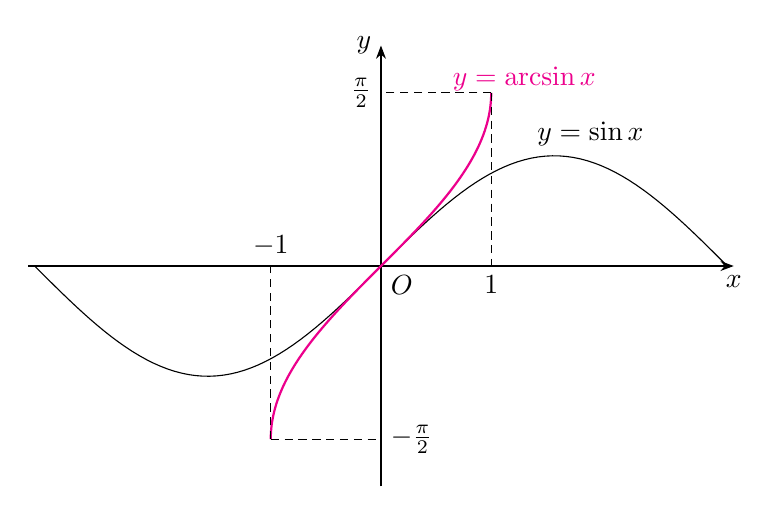
\begin{tikzpicture}[samples=100,scale=1.4]
\draw[-Stealth](-3.2,0)--(0,0)node[below right]{$O$}--(3.2,0)node[below]{$x$};
\draw[-Stealth](0,-2)--(0,2)node[left]{$y$};
\draw[domain=-pi:pi]plot(\x,{sin(\x r)});
\draw[semithick,domain=-pi/2:pi/2,draw=magenta,thick]plot({sin(\x r)},\x);
\node at(1.9,1.2){$y=\sin x$};\node[color=magenta] at(1.3,1.7){$y=\arcsin x$};
\draw[densely dashed](1,pi/2)--(1,0)node[below]{$1$}
(1,pi/2)--(0,pi/2)node[left]{$\frac\pi2$};
\draw[densely dashed](-1,-pi/2)--(-1,0)node[above]{$-1$}
(-1,-pi/2)--(0,-pi/2)node[right]{$-\frac\pi2$};
\end{tikzpicture}
  \end{lstlisting}
\end{minipage}
\hfil
\begin{minipage}[c]{0.45\textwidth}
  \centering
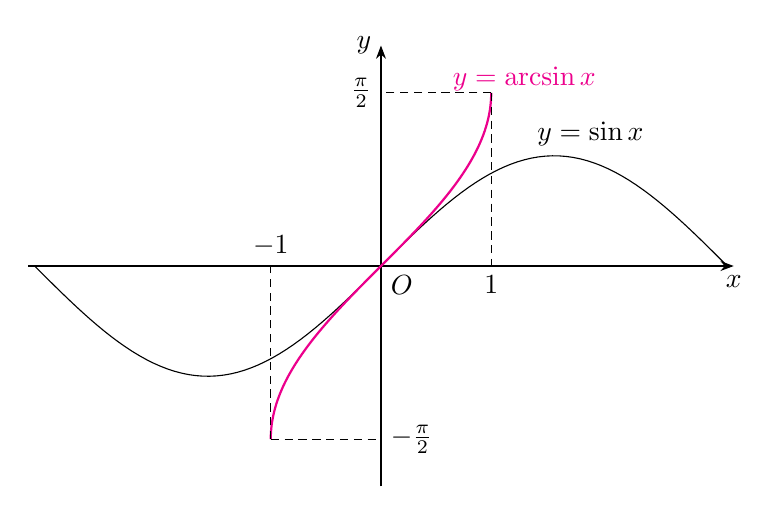
\begin{tikzpicture}[samples=100,scale=1.4]
\draw[-Stealth](-3.2,0)--(0,0)node[below right]{$O$}--(3.2,0)node[below]{$x$};
\draw[-Stealth](0,-2)--(0,2)node[left]{$y$};
\draw[domain=-pi:pi]plot(\x,{sin(\x r)});
\draw[semithick,domain=-pi/2:pi/2,draw=magenta,thick]plot({sin(\x r)},\x);
\node at(1.9,1.2){$y=\sin x$};\node[color=magenta] at(1.3,1.7){$y=\arcsin x$};
\draw[densely dashed](1,pi/2)--(1,0)node[below]{$1$}
(1,pi/2)--(0,pi/2)node[left]{$\frac\pi2$};
\draw[densely dashed](-1,-pi/2)--(-1,0)node[above]{$-1$}
(-1,-pi/2)--(0,-pi/2)node[right]{$-\frac\pi2$};
\end{tikzpicture}
\end{minipage}

  \item 反余弦函数

   \begin{minipage}[c]{0.485\textwidth}
  \centering
  \begin{lstlisting}[gobble=0]
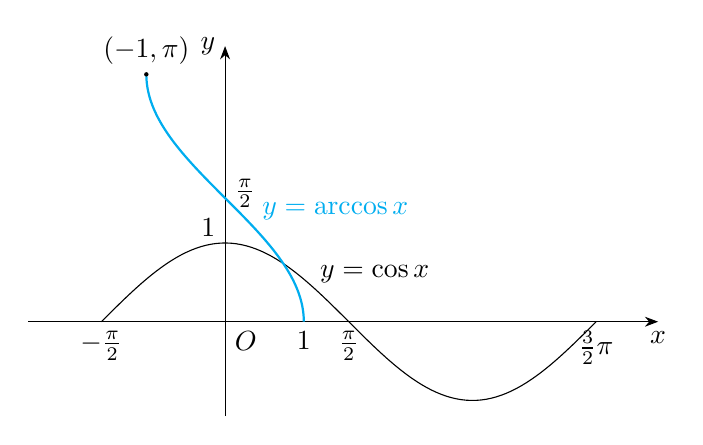
\begin{tikzpicture}[samples=100]
\draw[-Stealth](-2.5,0)--(0,0)node[below right]{$O$}--(5.5,0)node[below]{$x$};
\draw[-Stealth](0,-1.2)--(0,3.5)node[left]{$y$};
\draw[domain=-pi/2:3*pi/2]plot(\x,{cos(\x r)});\node[color=cyan] at(1.4,1.4){$y=\arccos x$};
\draw[semithick,domain=0:pi,thick,draw=cyan]plot({cos(\x r)},\x);
\node at(1.9,0.6){$y=\cos x$};
\node[left]at(0,1.2){$1$};\
\node[below] at(-pi/2,0){$-\frac\pi2$};
\node[below]at(pi/2,0){$\frac\pi2$};
\node[below]at(1,0){$1$};\node[right]at(0,1.63){$\frac\pi2$};
\node[below]at(3*pi/2,0){$\frac32\pi$};
\fill(-1,pi)circle(0.8pt)node[above]{$(-1,\pi)$};
\end{tikzpicture}
  \end{lstlisting}
\end{minipage}
\hfil
\begin{minipage}[c]{0.45\textwidth}
  \centering
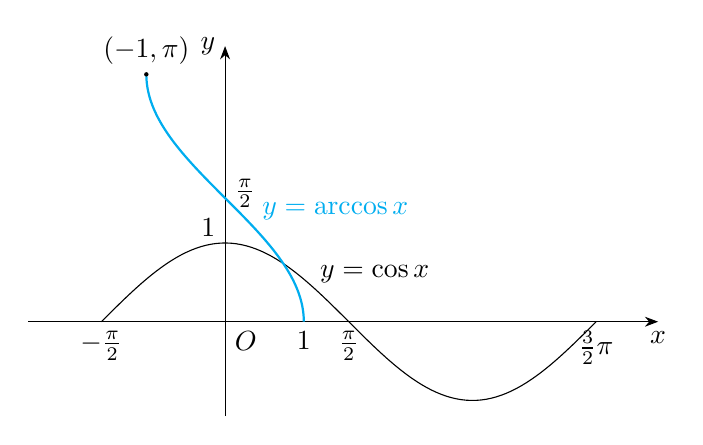
\begin{tikzpicture}[samples=100]
\draw[-Stealth](-2.5,0)--(0,0)node[below right]{$O$}--(5.5,0)node[below]{$x$};
\draw[-Stealth](0,-1.2)--(0,3.5)node[left]{$y$};
\draw[domain=-pi/2:3*pi/2]plot(\x,{cos(\x r)});\node[color=cyan] at(1.4,1.4){$y=\arccos x$};
\draw[semithick,domain=0:pi,thick,draw=cyan]plot({cos(\x r)},\x);
\node at(1.9,0.6){$y=\cos x$};
\node[left]at(0,1.2){$1$};\
\node[below] at(-pi/2,0){$-\frac\pi2$};
\node[below]at(pi/2,0){$\frac\pi2$};
\node[below]at(1,0){$1$};\node[right]at(0,1.63){$\frac\pi2$};
\node[below]at(3*pi/2,0){$\frac32\pi$};
\fill(-1,pi)circle(0.8pt)node[above]{$(-1,\pi)$};
\end{tikzpicture}
\end{minipage}

  \item 反正切函数

\begin{minipage}[c]{0.485\textwidth}
  \centering
  \begin{lstlisting}[gobble=0]
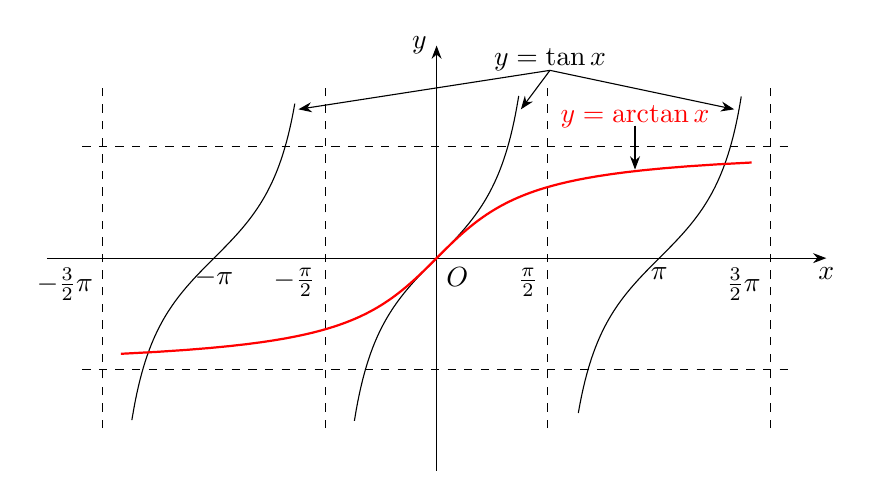
\begin{tikzpicture}[samples=100,scale=0.9]
\draw[-Stealth](-5.5,0)--(0,0)node[below right]{$O$}--(5.5,0)node[below]{$x$};
\draw[-Stealth](0,-3)--(0,3)node[left]{$y$};
\draw[domain=-4.3:-2]plot(\x,{tan(\x r)});
\draw[dashed](-3*pi/2,-2.4)--(-3*pi/2,2.4);
\draw[dashed](-pi/2,-2.4)--(-pi/2,2.4);
\draw[dashed](pi/2,-2.4)--(pi/2,2.4);
\draw[dashed](3*pi/2,-2.4)--(3*pi/2,2.4);
\draw[domain=-1.16:1.16]plot(\x,{tan(\x r)});
\draw[domain=2:4.3]plot(\x,{tan(\x r)});
\node[below left]at(-3*pi/2,0){$-\frac32\pi$};
\node[below left]at(3*pi/2,0){$\frac32\pi$};
\node[below left]at(pi/2,0){$\frac\pi2$};\node[below left]at(-pi/2,0){$-\frac\pi2$};
\node[below]at(pi,0){$\pi$};\node[below]at(-pi,0){$-\pi$};
\node(a)at(1.6,2.8){$y=\tan x$};\node[color=red](b) at(2.8,2){$y=\arctan x$};
\draw[semithick,domain=-1.35:1.35,thick,draw=red]plot({tan(\x r)},\x);
\draw[dashed](-5,pi/2)--(5,pi/2)(-5,-pi/2)--(5,-pi/2);
\draw[-Stealth](2.8,1.87)--(2.8,1.25);
\draw[-Stealth](1.6,2.65)--(-1.95,2.1);
\draw[-Stealth](1.6,2.65)--(1.19,2.1);\draw[-Stealth](1.6,2.65)--(4.2,2.1);
\end{tikzpicture}
  \end{lstlisting}
\end{minipage}
\hfil
\begin{minipage}[c]{0.45\textwidth}
  \centering
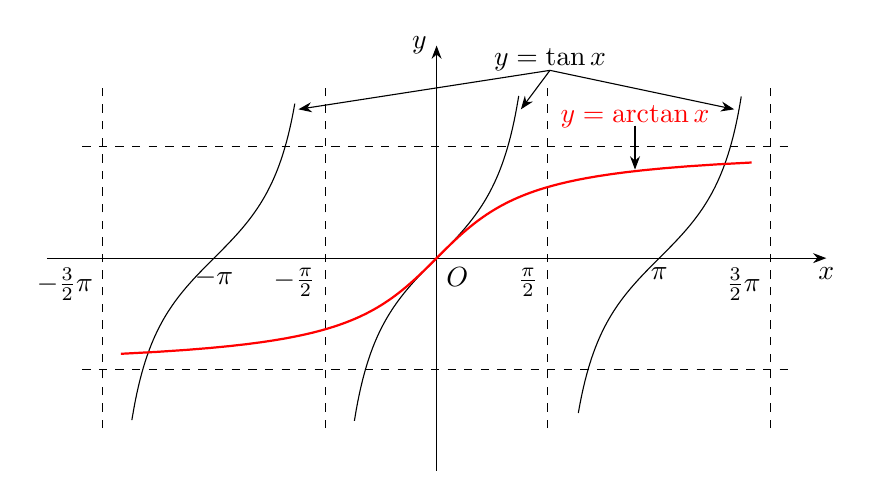
\begin{tikzpicture}[samples=100,scale=0.9]
\draw[-Stealth](-5.5,0)--(0,0)node[below right]{$O$}--(5.5,0)node[below]{$x$};
\draw[-Stealth](0,-3)--(0,3)node[left]{$y$};
\draw[domain=-4.3:-2]plot(\x,{tan(\x r)});
\draw[dashed](-3*pi/2,-2.4)--(-3*pi/2,2.4);
\draw[dashed](-pi/2,-2.4)--(-pi/2,2.4);
\draw[dashed](pi/2,-2.4)--(pi/2,2.4);
\draw[dashed](3*pi/2,-2.4)--(3*pi/2,2.4);
\draw[domain=-1.16:1.16]plot(\x,{tan(\x r)});
\draw[domain=2:4.3]plot(\x,{tan(\x r)});
\node[below left]at(-3*pi/2,0){$-\frac32\pi$};
\node[below left]at(3*pi/2,0){$\frac32\pi$};
\node[below left]at(pi/2,0){$\frac\pi2$};\node[below left]at(-pi/2,0){$-\frac\pi2$};
\node[below]at(pi,0){$\pi$};\node[below]at(-pi,0){$-\pi$};
\node(a)at(1.6,2.8){$y=\tan x$};\node[color=red](b) at(2.8,2){$y=\arctan x$};
\draw[semithick,domain=-1.35:1.35,thick,draw=red]plot({tan(\x r)},\x);
\draw[dashed](-5,pi/2)--(5,pi/2)(-5,-pi/2)--(5,-pi/2);
\draw[-Stealth](2.8,1.87)--(2.8,1.25);
\draw[-Stealth](1.6,2.65)--(-1.95,2.1);
\draw[-Stealth](1.6,2.65)--(1.19,2.1);\draw[-Stealth](1.6,2.65)--(4.2,2.1);
\end{tikzpicture}
\end{minipage}


\end{enumerate}



\subsection{圆锥曲线的~TikZ 绘制}

圆锥曲线的产生


\lstinputlisting[style=latex, firstline=1]{figures/yuanzhuiquxian.tex}

\begin{minipage}[c]{\linewidth}
  \centering
 \includegraphics[width=\linewidth]{yuanzhuiquxian}
\end{minipage}


\begin{enumerate}
  \item 在坐标系中的圆

\begin{minipage}[c]{0.485\textwidth}
  \centering
  \begin{lstlisting}[gobble=0]
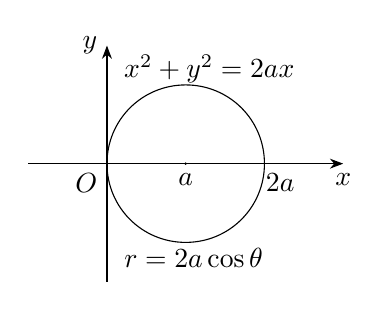
\begin{tikzpicture}[samples=100]
\draw[-Stealth](-1,0)--(0,0)node[below left]{$O$}--(3,0)node[below]{$x$};
\draw[-Stealth](0,-1.5)--(0,1.5)node[left]{$y$};
\draw plot[tension=1,smooth cycle]coordinates{(0,0)(1,1)(2,0)(1,-1)};
\node [below]at(2.2,0){$2a$};\node [below]at(1,0){$a$};
\fill(1,0)circle(0.5pt);
\node at(1.1,-1.2){$r=2a\cos\theta$};
\node at(1.3,1.2){$x^2+y^2=2ax$};
\end{tikzpicture}
  \end{lstlisting}
\end{minipage}
\hfil
\begin{minipage}[c]{0.45\textwidth}
  \centering
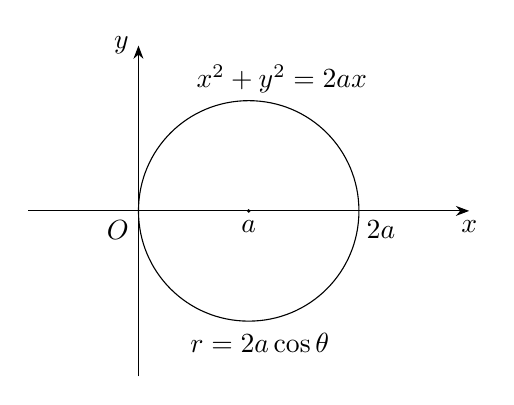
\begin{tikzpicture}[samples=100,scale=1.4]
\draw[-Stealth](-1,0)--(0,0)node[below left]{$O$}--(3,0)node[below]{$x$};
\draw[-Stealth](0,-1.5)--(0,1.5)node[left]{$y$};
\draw plot[tension=1,smooth cycle]coordinates{(0,0)(1,1)(2,0)(1,-1)};
\node [below]at(2.2,0){$2a$};\node [below]at(1,0){$a$};
\fill(1,0)circle(0.5pt);
\node at(1.1,-1.2){$r=2a\cos\theta$};
\node at(1.3,1.2){$x^2+y^2=2ax$};
\end{tikzpicture}
\end{minipage}

  \item 椭圆的图像绘制

  \begin{minipage}[c]{0.485\textwidth}
  \centering
  \begin{lstlisting}[gobble=0]
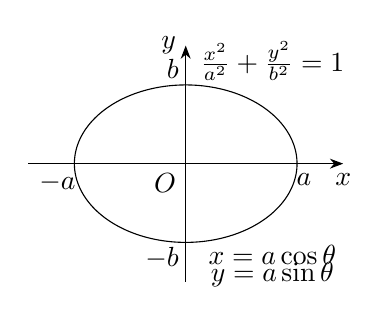
\begin{tikzpicture}[samples=200]
\draw[-Stealth](-2,0)--(0,0)node[below left]{$O$}--(2,0)node[below]{$x$};
\draw[-Stealth](0,-1.5)--(0,1.5)node[left]{$y$};
\draw[domain=0:2*pi]plot({1.414*cos(\x r)},{sin(\x r)});
\node[left=-1pt] at(0,1.2){$b$};\node[left=-1pt] at(0,-1.2){$-b$};
\node[below] at(-1.63,0){$-a$};\node[below] at(1.5,0){$a$};
\node at(1.1,1.3){$\frac{x^2}{a^2}+\frac{y^2}{b^2}=1$};
\node[align=flush center] at(1.1,-1.3){$x=a\cos\theta$\\[-2mm]
$y=a\sin\theta$};
\end{tikzpicture}
  \end{lstlisting}
\end{minipage}
\hfil
\begin{minipage}[c]{0.45\textwidth}
  \centering
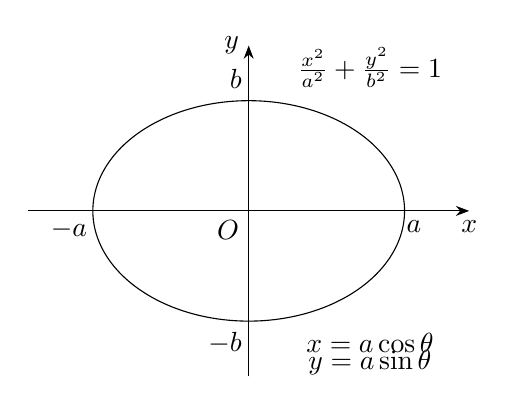
\begin{tikzpicture}[samples=200,scale=1.4]
\draw[-Stealth](-2,0)--(0,0)node[below left]{$O$}--(2,0)node[below]{$x$};
\draw[-Stealth](0,-1.5)--(0,1.5)node[left]{$y$};
\draw[domain=0:2*pi]plot({1.414*cos(\x r)},{sin(\x r)});
\node[left=-1pt] at(0,1.2){$b$};\node[left=-1pt] at(0,-1.2){$-b$};
\node[below] at(-1.63,0){$-a$};\node[below] at(1.5,0){$a$};
\node at(1.1,1.3){$\frac{x^2}{a^2}+\frac{y^2}{b^2}=1$};
\node[align=flush center] at(1.1,-1.3){$x=a\cos\theta$\\[-2mm]
$y=a\sin\theta$};
\end{tikzpicture}
\end{minipage}



  \item 双曲线的~tizk 实现

\begin{minipage}[c]{0.485\textwidth}
  \centering
  \begin{lstlisting}[gobble=0]
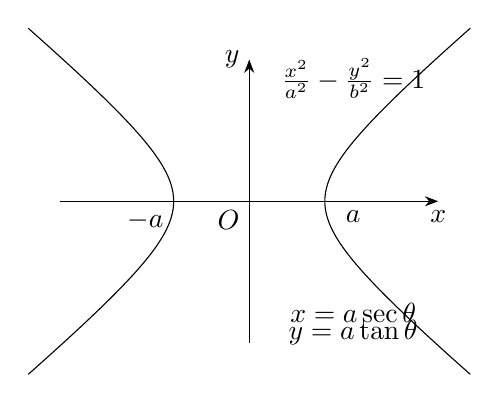
\begin{tikzpicture}[samples=200,scale=1.2]
\def\a{0.8}
\def\b{2/3}
\draw[-Stealth](-2,0)--(0,0)node[below left]{$O$}--(2,0)node[below]{$x$};
\draw[-Stealth](0,-1.5)--(0,1.5)node[left]{$y$};
\draw[domain=-70:70] plot ({\a*sec(\x)},{\b*tan(\x)});
\draw[domain=110:250] plot ({\a*sec(\x)},{\b*tan(\x)});
\node[below] at(-1.1,0){$-a$};\node[below] at(1.1,0){$a$};
\node at(1.1,1.3){$\frac{x^2}{a^2}-\frac{y^2}{b^2}=1$};
\node[align=flush center] at(1.1,-1.3){$x=a\sec\theta$\\[-2mm]
$y=a\tan\theta$};
\end{tikzpicture}
  \end{lstlisting}
\end{minipage}
\hfil
\begin{minipage}[c]{0.45\textwidth}
  \centering
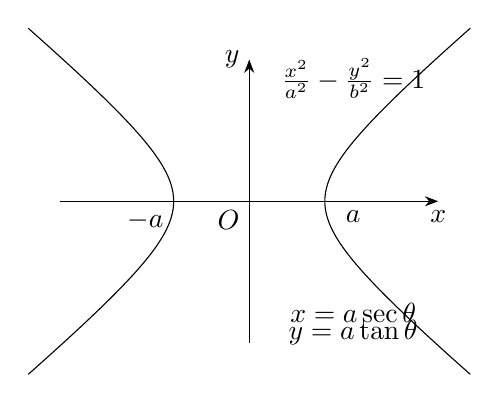
\begin{tikzpicture}[samples=200,scale=1.2]
\def\a{0.8}
\def\b{2/3}
\draw[-Stealth](-2,0)--(0,0)node[below left]{$O$}--(2,0)node[below]{$x$};
\draw[-Stealth](0,-1.5)--(0,1.5)node[left]{$y$};
\draw[domain=-70:70] plot ({\a*sec(\x)},{\b*tan(\x)});
\draw[domain=110:250] plot ({\a*sec(\x)},{\b*tan(\x)});
\node[below] at(-1.1,0){$-a$};\node[below] at(1.1,0){$a$};
\node at(1.1,1.3){$\frac{x^2}{a^2}-\frac{y^2}{b^2}=1$};
\node[align=flush center] at(1.1,-1.3){$x=a\sec\theta$\\[-2mm]
$y=a\tan\theta$};
\end{tikzpicture}
\end{minipage}


\item 抛物线的绘制

\begin{minipage}[c]{0.485\textwidth}
  \centering
  \begin{lstlisting}[gobble=0]
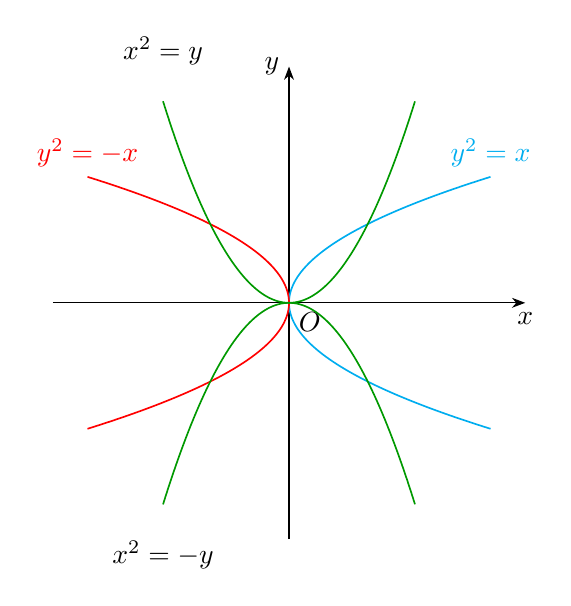
\begin{tikzpicture}[samples=100]
\draw[-Stealth](-3,0)--(0,0)node[below right]{$O$}--(3,0)node[below]{$x$};
\draw[-Stealth](0,-3)--(0,3)node[left]{$y$};
\draw[semithick,domain=0:1.6,draw=cyan]plot({(\x)^2},\x)
node[above,color=cyan]{$y^2=x$};
\draw[semithick,domain=0:1.6,draw=red]plot({-(\x)^2},\x)
node[above,color=red]{$y^2=-x$};
\draw[semithick,domain=0:1.6,draw=cyan]plot({(\x)^2},-\x);
\draw[semithick,domain=0:1.6,draw=red]plot({-(\x)^2},-\x);
\draw[semithick,domain=-1.6:1.6,draw=green!60!black]plot(\x,{(\x)^2});
\node at(-1.6,3.2){$x^2=y$};
\draw[semithick,domain=-1.6:1.6,draw=green!60!black]plot(\x,{-(\x)^2});
\node at(-1.6,-3.2){$x^2=-y$};
\end{tikzpicture}
  \end{lstlisting}
\end{minipage}
\hfil
\begin{minipage}[c]{0.45\textwidth}
  \centering
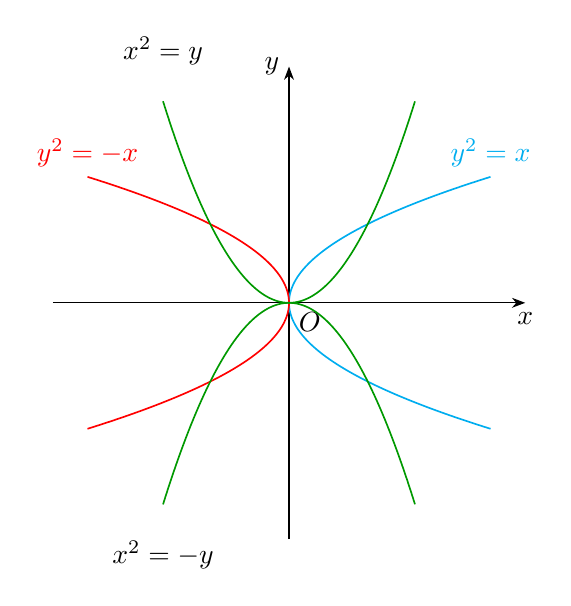
\begin{tikzpicture}[samples=100]
\draw[-Stealth](-3,0)--(0,0)node[below right]{$O$}--(3,0)node[below]{$x$};
\draw[-Stealth](0,-3)--(0,3)node[left]{$y$};
\draw[semithick,domain=0:1.6,draw=cyan]plot({(\x)^2},\x)
node[above,color=cyan]{$y^2=x$};
\draw[semithick,domain=0:1.6,draw=red]plot({-(\x)^2},\x)
node[above,color=red]{$y^2=-x$};
\draw[semithick,domain=0:1.6,draw=cyan]plot({(\x)^2},-\x);
\draw[semithick,domain=0:1.6,draw=red]plot({-(\x)^2},-\x);
\draw[semithick,domain=-1.6:1.6,draw=green!60!black]plot(\x,{(\x)^2});
\node at(-1.6,3.2){$x^2=y$};
\draw[semithick,domain=-1.6:1.6,draw=green!60!black]plot(\x,{-(\x)^2});
\node at(-1.6,-3.2){$x^2=-y$};
\end{tikzpicture}
\end{minipage}


\end{enumerate}



\subsection{图像阴影填充面积与定积分}

\begin{enumerate}
  \item 不等式的“穿针引线”法

  \begin{minipage}[c]{0.485\linewidth}
   \lstinputlisting[style=latex, firstline=9,lastline=17]{figures/ZGF.tex}
\end{minipage}
\begin{minipage}[c]{0.485\linewidth}
  \centering
 \includegraphics[scale=1.2]{ZGF}
\end{minipage}

\item 线性规划

   \lstinputlisting[style=latex,firstline=1,lastline=20]{figures/yinying2.tex}

{\centering
   \includegraphics[scale=1]{yinying2}
}

\begin{minipage}[c]{0.485\linewidth}
   \lstinputlisting[style=latex, firstline=1,lastline=25]{figures/yinying.tex}
\end{minipage}
\begin{minipage}[c]{0.485\linewidth}
  \centering
 \includegraphics[scale=1]{yinying}
\end{minipage}

\item 定积分

   \lstinputlisting[style=latex,firstline=27,lastline=44]{figures/SCTfonction2.tex}

{\centering
   \includegraphics[scale=2]{SCTfonction2-1}
}


   \lstinputlisting[style=latex,firstline=48,lastline=70]{figures/SCTfonction2.tex}

{\centering
   \includegraphics[scale=2]{SCTfonction2-2}
}

   \lstinputlisting[style=latex,firstline=73,lastline=92]{figures/SCTfonction2.tex}

{\centering
   \includegraphics[scale=1.5]{SCTfonction2-3}
}

   \lstinputlisting[style=latex,firstline=96,lastline=115]{figures/SCTfonction2.tex}

{\centering
   \includegraphics[scale=2]{SCTfonction2-4}
}




   \lstinputlisting[style=latex,firstline=1,lastline=28]{figures/integrate2.tex}

\begin{minipage}[c]{0.485\linewidth}
   \includegraphics[scale=1]{integrate2}\\
\end{minipage}\hfill
\begin{minipage}[c]{0.485\linewidth}
  \centering
\includegraphics[scale=1]{integrate3}
\end{minipage}


\lstinputlisting[style=latex,firstline=1,lastline=14]{figures/integrate3.tex}

\end{enumerate}



\begin{minipage}[c]{0.485\linewidth}
   \lstinputlisting[style=latex, firstline=9,lastline=15]{figures/Integrate.tex}
\end{minipage}
\begin{minipage}[c]{0.485\linewidth}
  \centering
 \includegraphics[scale=1]{Integrate}
\end{minipage}

\section{统计图的~TikZ 绘制}

\subsection{折线图的~TikZ 绘制}

\subsection{柱状图的~TikZ 绘制}

\subsection{饼图的~TikZ 绘制}

\section{几何图形的~TikZ 绘制}

\subsection{平面几何图形的~TikZ 绘制}

\subsection{空间几何图形的~TikZ 绘制}

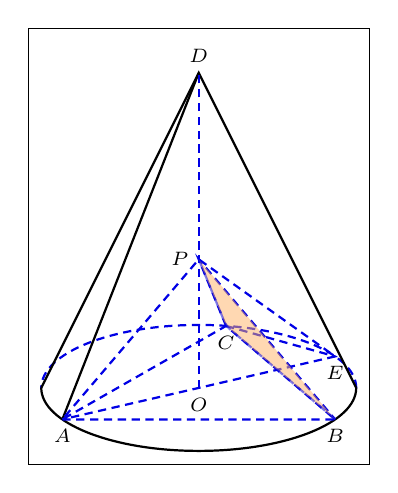
\begin{tikzpicture}[thick, framed,show background top,lines/.style=blue!90!black,scale=0.8]

\coordinate(O)at(0,0)node[below]{\scriptsize$O$};
\coordinate(A)at(-2.165,-0.5);
\coordinate(B)at(2.165,-0.5);
\coordinate(C)at(0.434,0.984);%%\theta=80
\coordinate(E)at(2.165,0.5);
\coordinate(D)at(0,5);
\coordinate(P)at(0,2.041);
\coordinate(F)at(-2.5,0);
\coordinate(G)at(2.5,0);


\draw[densely dashed,lines](2.5,0)arc[start angle=0,end angle=180,x radius=2.5,y radius=1];
\draw(2.5,0)arc[start angle=0,end angle=-180,x radius=2.5,y radius=1];
\draw (F)--(D)--(G);
\draw(A)--(D);
\draw[densely dashed,lines](A)--(B)--(C)--(A)--(P)--(E)--(A);
\draw[densely dashed,lines](C)--(P)--(B);
\draw[densely dashed,lines](O)--(D);
\draw[densely dashed,lines](C)--(E);

\node at (A)[below]{\scriptsize$A$};
\node at (B)[below]{\scriptsize$B$};
\node at(E)[below]{\scriptsize$E$};
\node at(D)[above]{\scriptsize$D$};
\node at(P)[left]{\scriptsize$P$};
\node at(C)[below]{\scriptsize$C$};

\draw [lines,densely dashed,rounded corners=2pt,opacity=0.5,fill=orange!60](P)--(C)--(B);
\end{tikzpicture}

\begin{minipage}[c]{\linewidth}
   \lstinputlisting[style=latex, firstline=6,lastline=23]{figures/Cone.tex}
\end{minipage}\hfill
\begin{minipage}[c]{\linewidth}
  \centering
 \includegraphics[width=\linewidth]{Cone}
\end{minipage}

\section{图像的大致图像的~TikZ 绘制}

\section{混合图形的~TikZ 绘制}

\section{PGFplots 实现杂例}

本手册中的图像是使用\textcolor{black}{Ti\textcolor{orange}{\emph{k}}Z}-\textcolor{blue}{network} library或Ti\emph{k}Z。 为每个图像指定用于此的代码。

\begin{minipage}[c]{0.51\textwidth}
  \centering
  \begin{lstlisting}[gobble=0]
        
\begin{tikzpicture}
         \filldraw (-.2,.2) circle (2pt)
          (.2,.2) circle (2pt);
         \draw (0,0) circle (5mm) (-.3,-.1) .. controls (0,-.3) ..(.3,-.1);
        \end{tikzpicture}
  \end{lstlisting}
\end{minipage}
\hfil
\begin{minipage}[c]{0.45\textwidth}
  \centering
  
\begin{tikzpicture}
    \filldraw (-.2,.2) circle (2pt) (.2,.2) circle (2pt);
    \draw (0,0) circle (5mm) (-.3,-.1) .. controls (0,-.3) ..
    (.3,-.1);
    \end{tikzpicture}
\end{minipage}








































% \input{versionhistory.tex}
% \vhListAllAuthorsLongWithAbbrev

\end{document} 